\newpage

{\setlength{\parskip}{0cm} {
\chapter*{Anexos}

\setlength{\parindent}{0ex}

\textbf{Anexo 1} \\
\textit{Modelo de la encuesta distribuida para el establecimiento de los métodos empleados por la población en la Urbanización Guaraguao de Puerto La Cruz}
}

\begin{figure}[!ht]
    \centering
    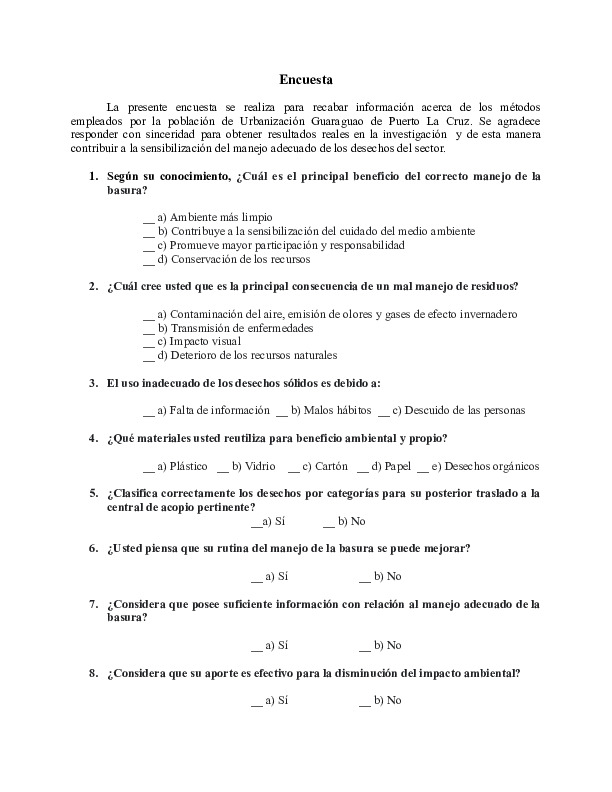
\includegraphics[width=13cm]{Media/Encuesta 1.jpg}
    \label{fig:encuesta}
\end{figure}

\setlength{\parindent}{0ex}

Fuente: Elaboración propia

\newpage

\setlength{\parindent}{0ex}

\textbf{Anexo 2} \\
\textit{Folleto entregado durante la campaña divulgativa realizada en la Urbanización Guaraguao de Puerto La Cruz}
}
\begin{figure}[!ht]
    \centering
    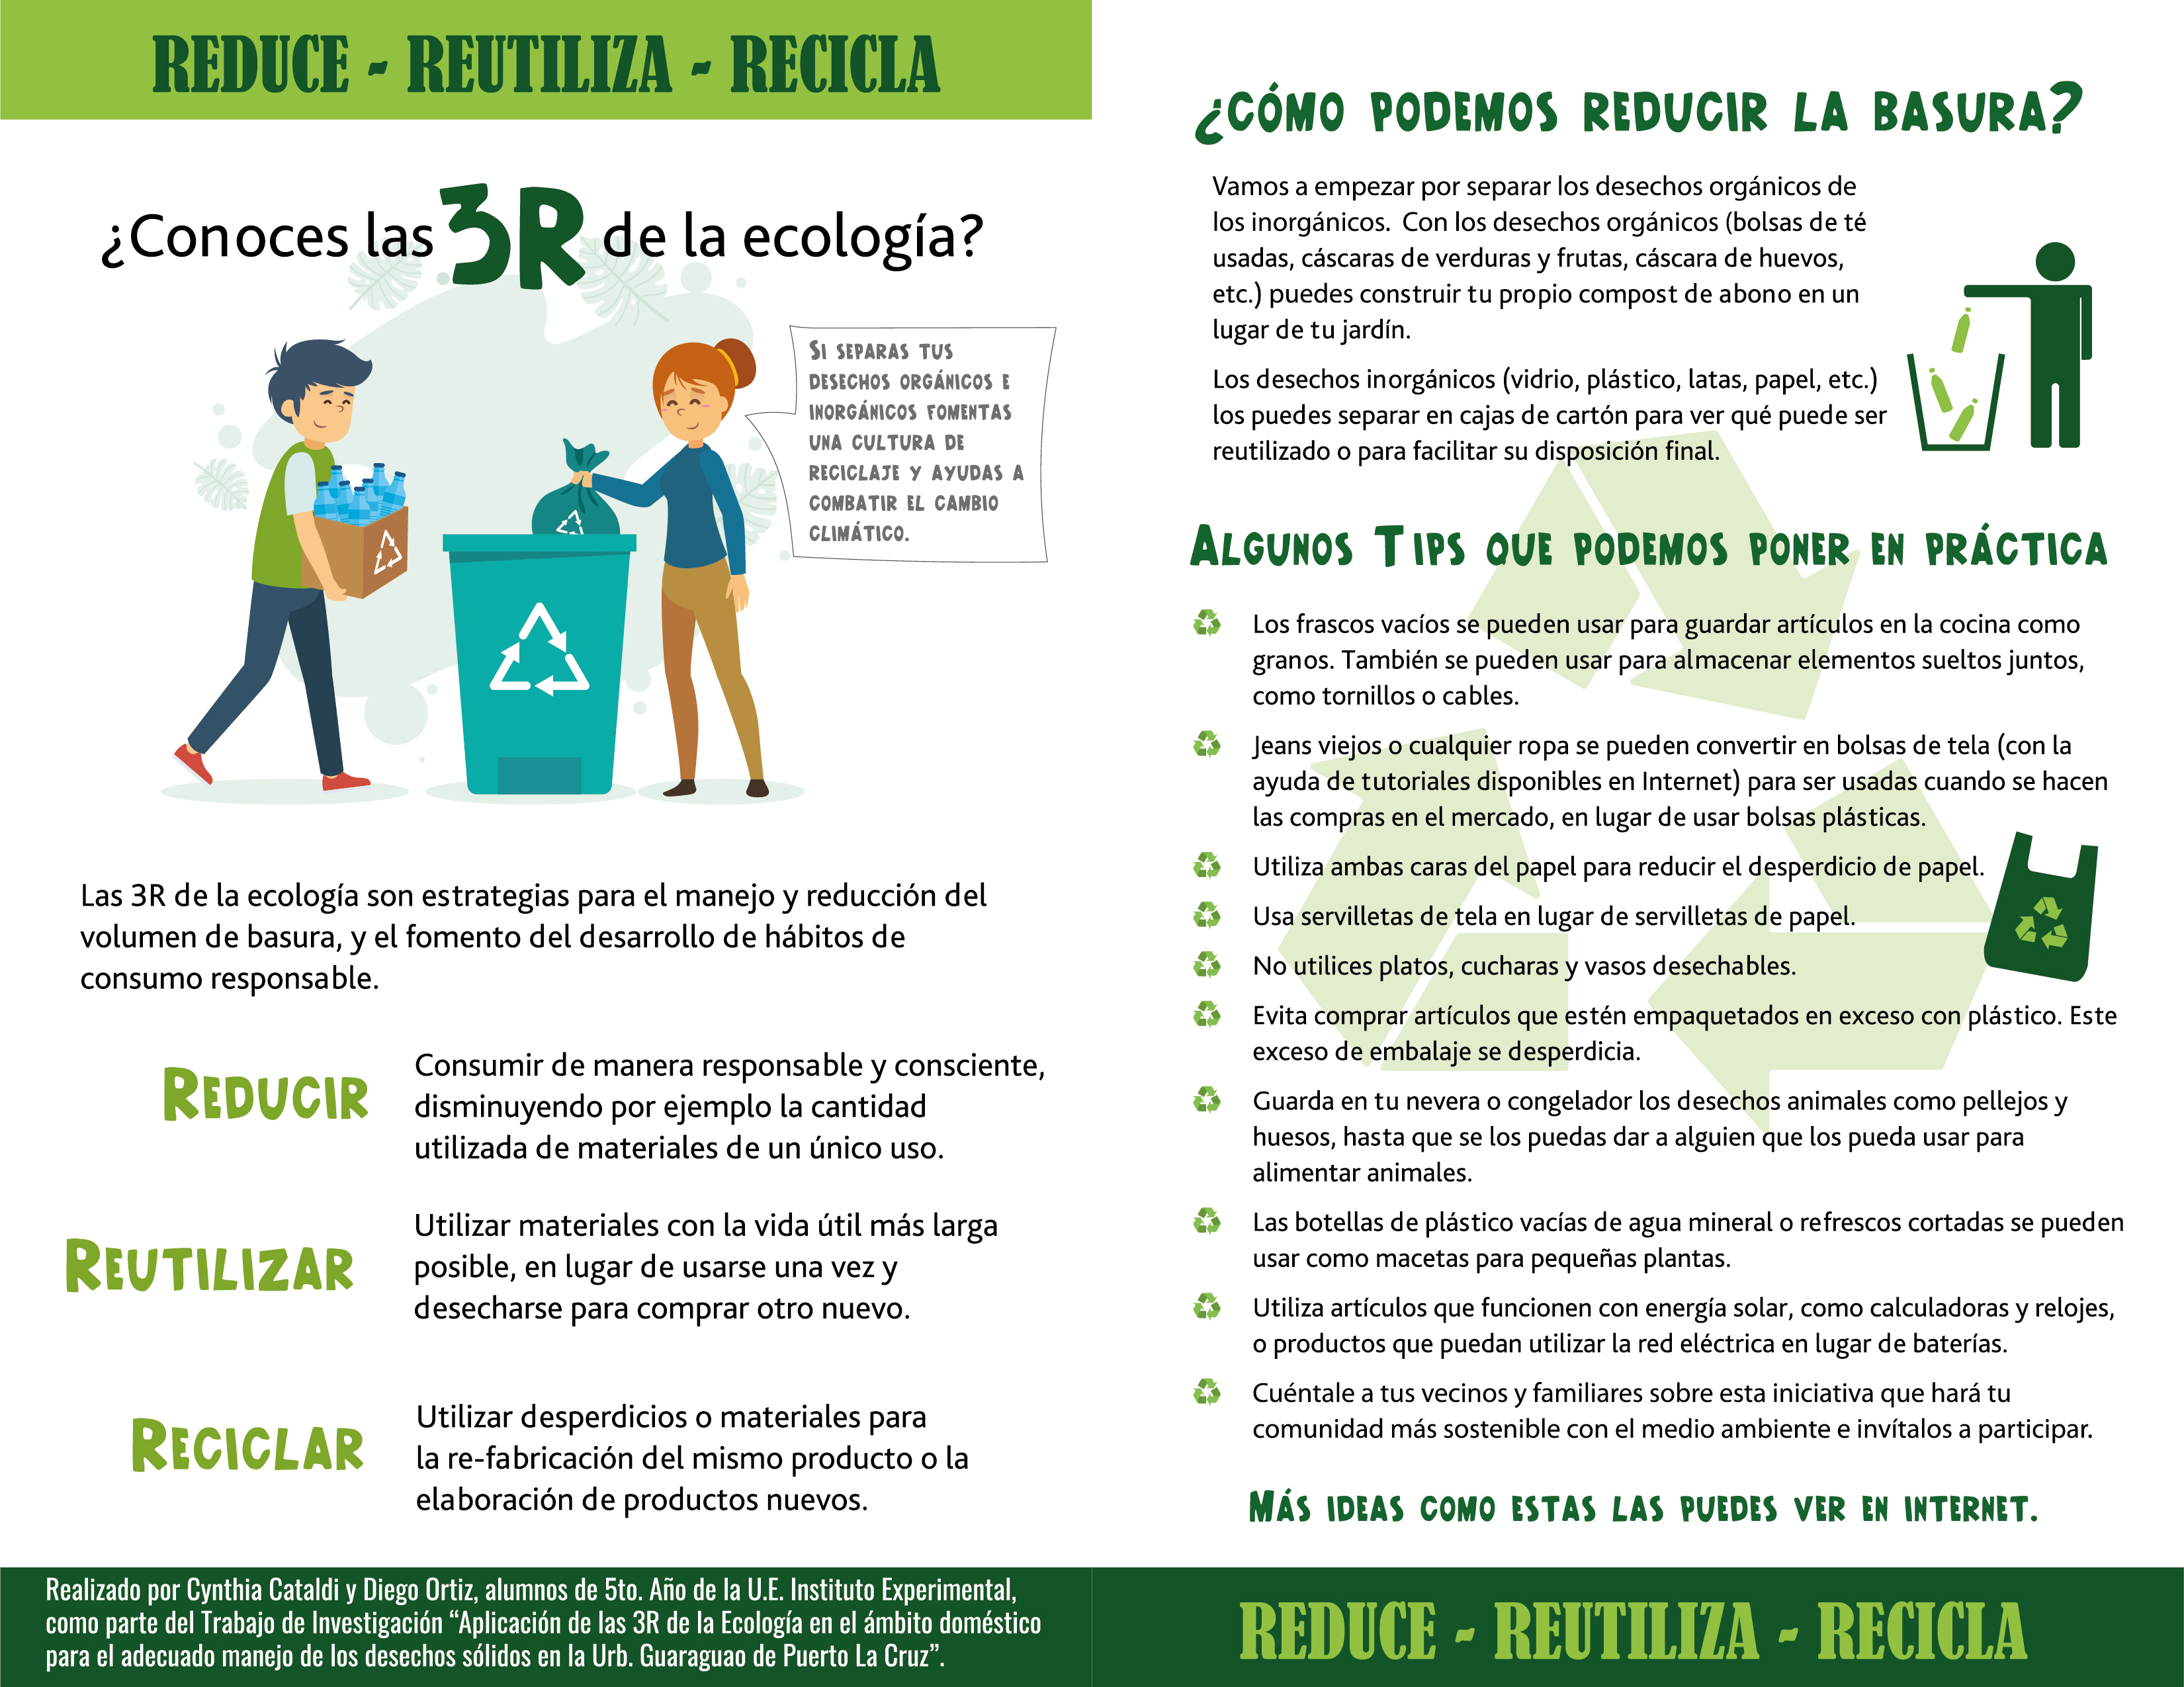
\includegraphics[width=17cm, angle=90]{Media/Volante.jpg}
    \label{fig:folleto}
\end{figure}

\setlength{\parindent}{0ex}

Fuente: Elaboración propia

\newpage

\setlength{\parindent}{0ex}

\textbf{Anexo 3} \\
\textit{Modelo de la encuesta distribuida para determinar los cambios en los hábitos del manejo de la basura a raíz de la campaña divulgativa realizada en la Urbanización Guaraguao de Puerto La Cruz}

\begin{figure}[!ht]
    \centering
    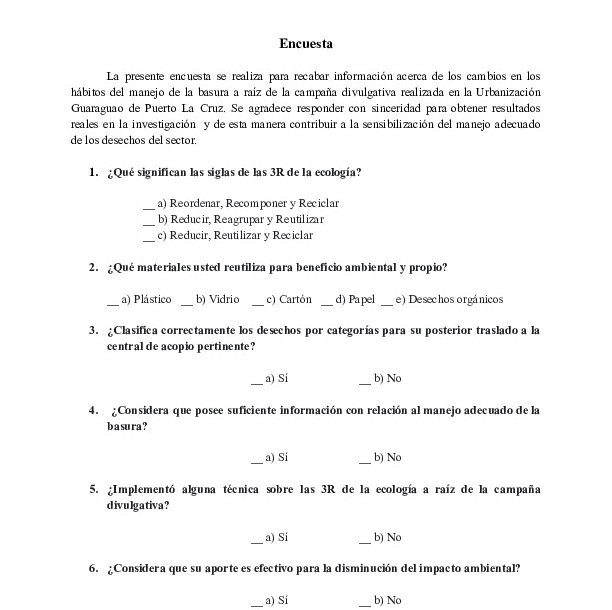
\includegraphics[width=15cm]{Media/Encuesta 2.jpg}
    \label{fig:encuesta2}
\end{figure}

\setlength{\parindent}{0ex}

Fuente: Elaboración propia

\newpage

\textbf{Anexo 4} \\
\textit{Lista de Cotejo realizada para el seguimiento de las estrategias propuestas para la aplicación de las 3R de la ecología en la Urbanización Guaraguao de Puerto La Cruz}

\begin{figure}[!ht]
    \centering
    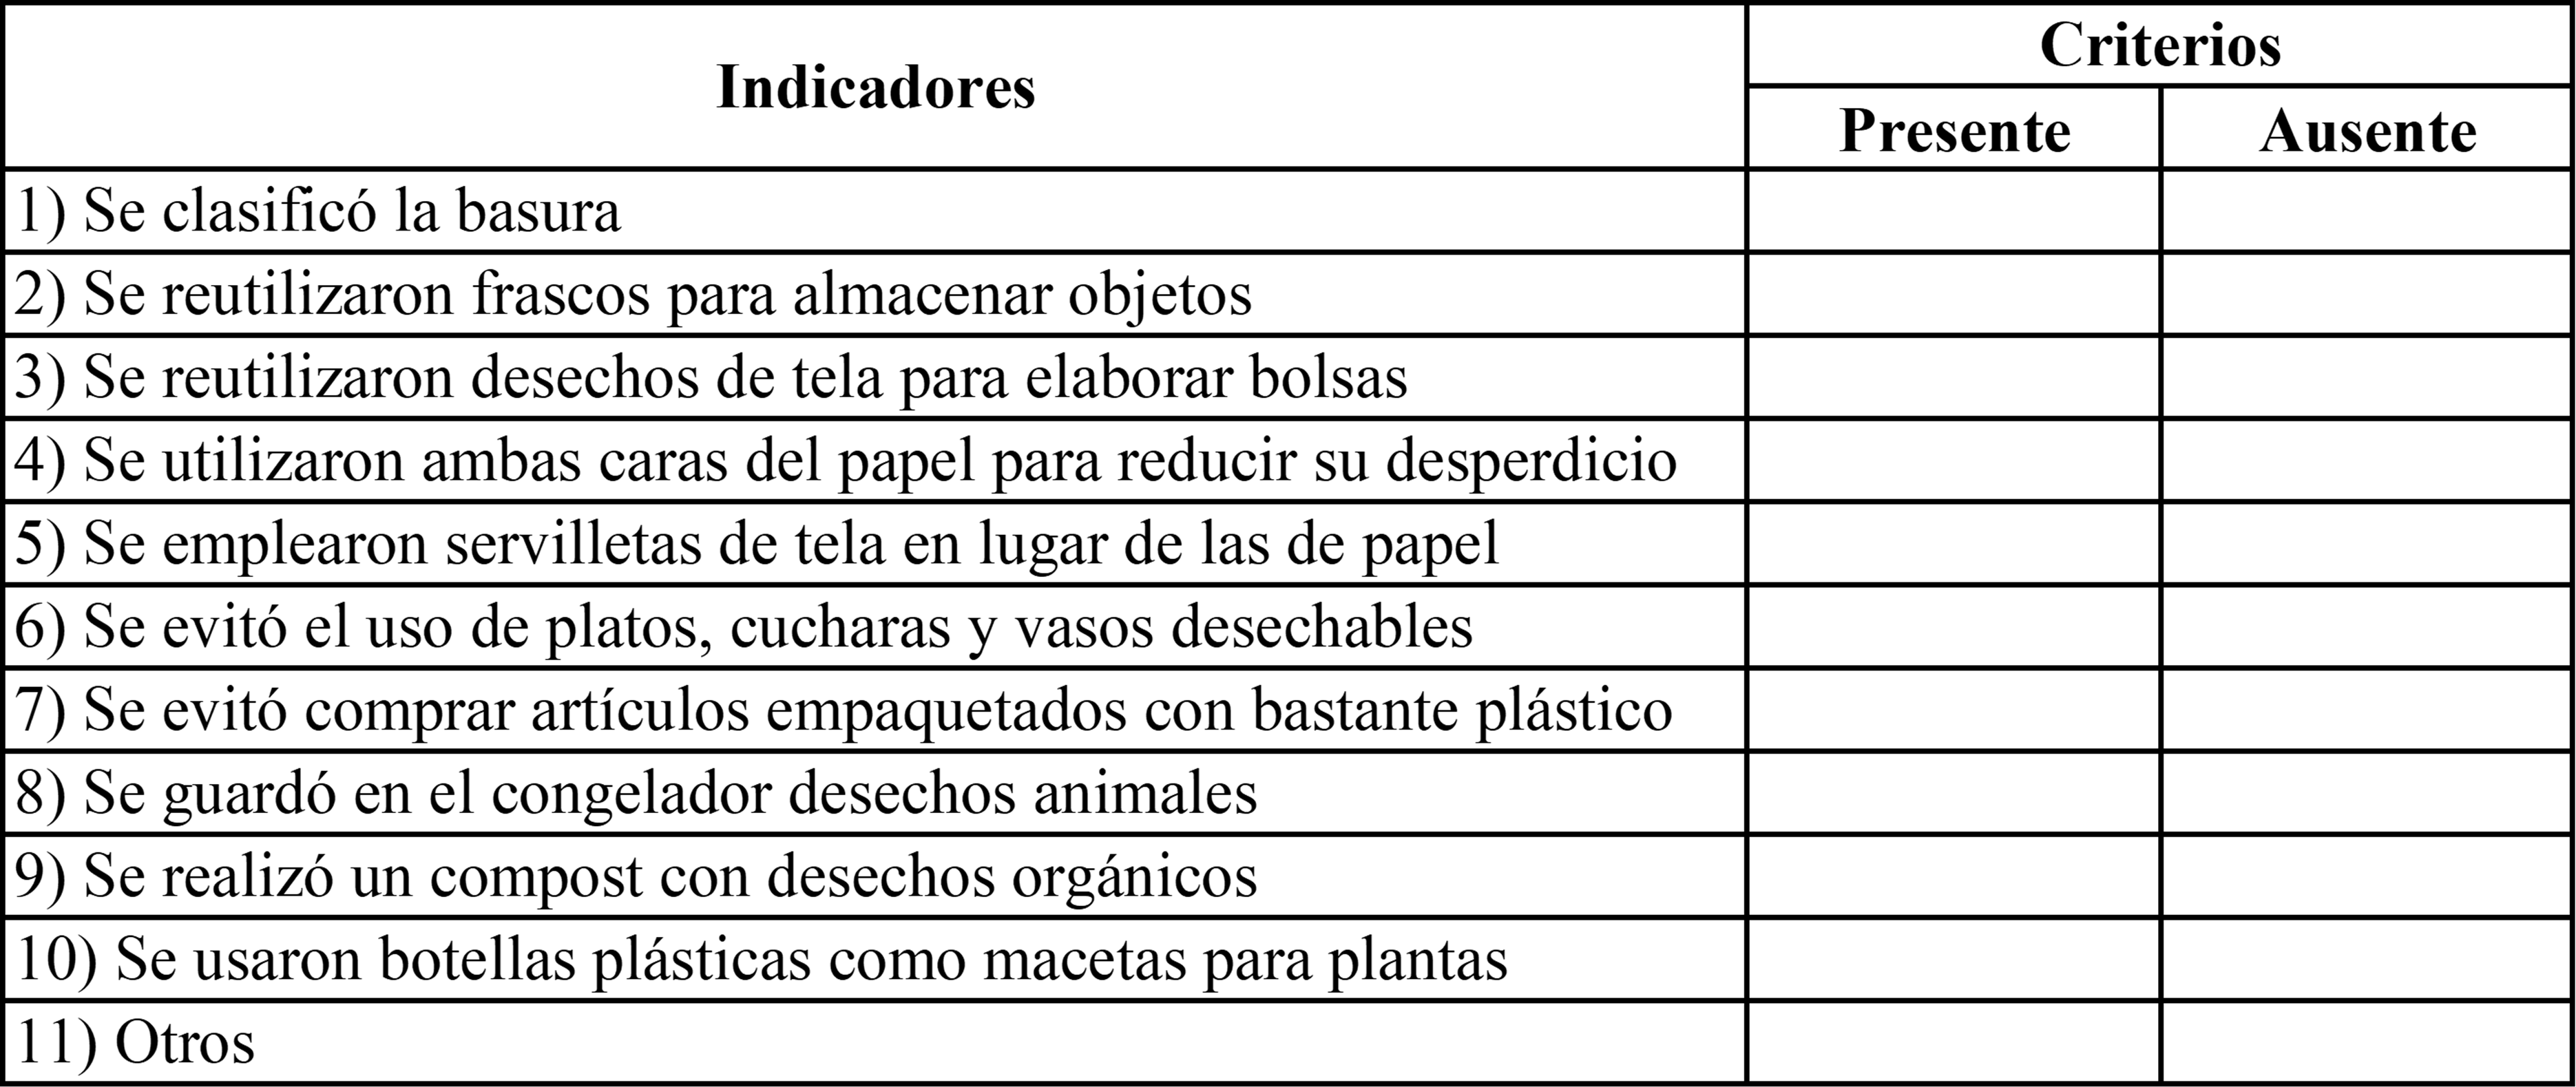
\includegraphics[width=15cm]{Media/lista de cotejo.png}
    \label{fig:ListadeCotejo}
\end{figure}

\setlength{\parindent}{0ex}

Fuente: Elaboración propia

\newpage

\textbf{Anexo 5} \\
\textit{Otras estrategias aplicadas por la muestra seleccionada para la aplicación de las 3R de la ecología}

\begin{figure}[!ht]
    \centering
    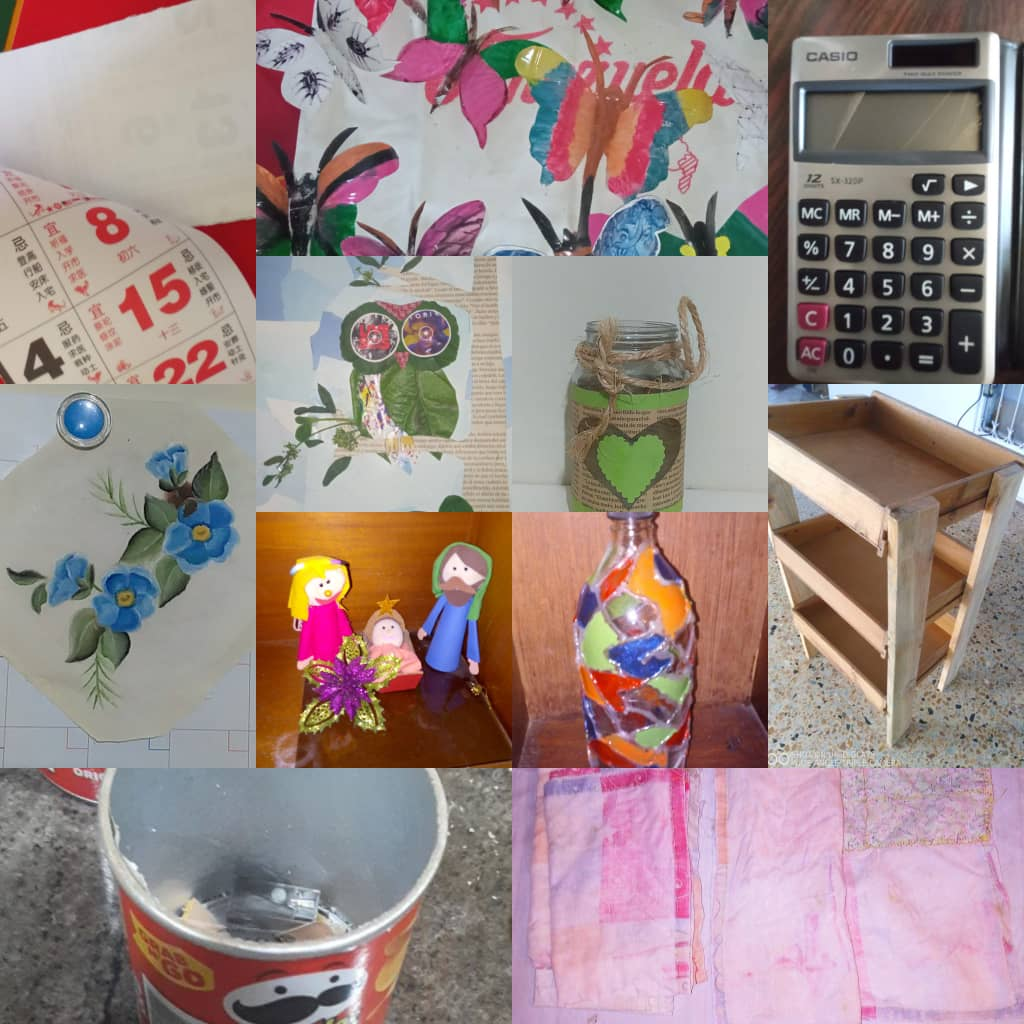
\includegraphics[width=15cm]{Media/Fotos/Foto 1 otros.jpeg}
    \label{fig:anexo5}
\end{figure}

\setlength{\parindent}{0ex}

Fuente: Elaboración propia

\newpage

\textbf{Anexo 6} \\
\textit{Estrategia de almacenar desechos animales en el congelador}

\begin{figure}[!ht]
    \centering
    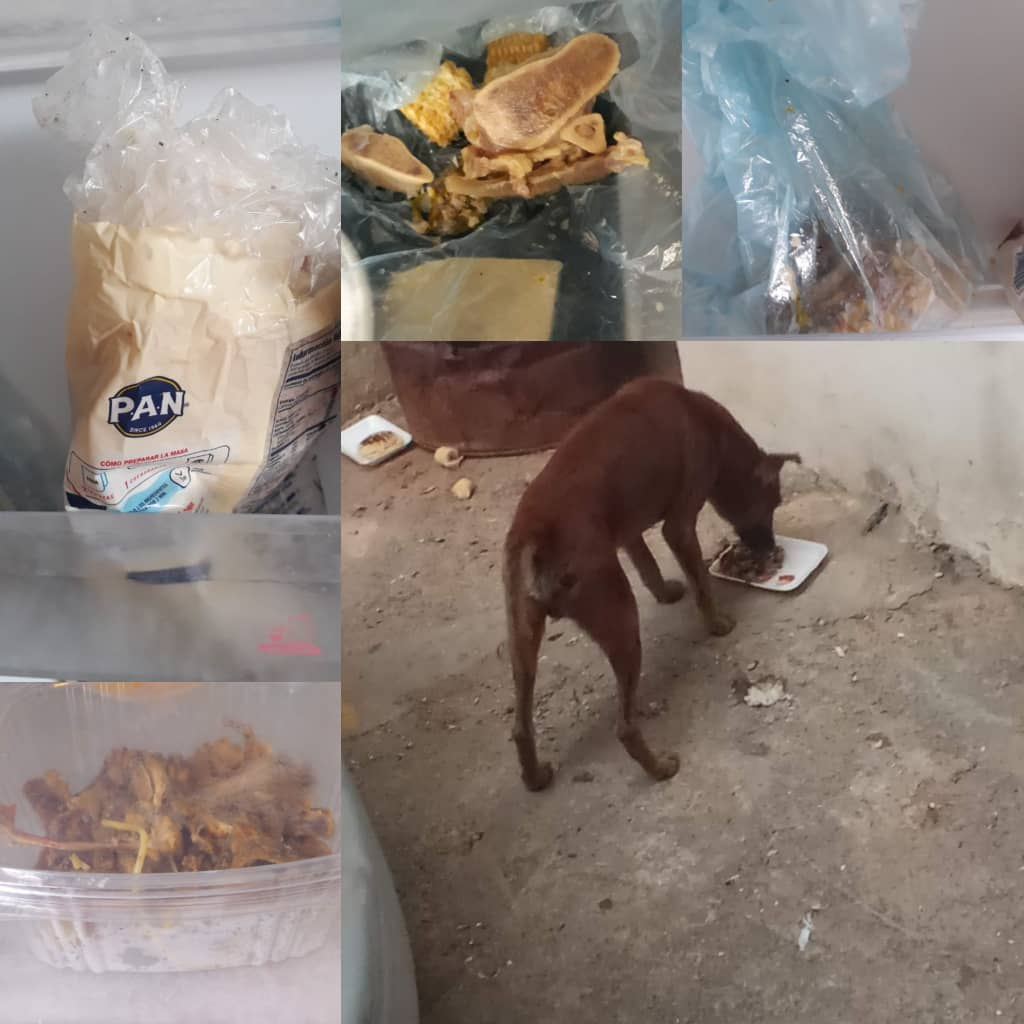
\includegraphics[width=15cm]{Media/Fotos/Foto 2 huesos.jpeg}
    \label{fig:anexo6}
\end{figure}

\setlength{\parindent}{0ex}

Fuente: Elaboración propia

\newpage

\textbf{Anexo 7} \\
\textit{Reutilización de envases para almacenar objetos}

\begin{figure}[!ht]
    \centering
    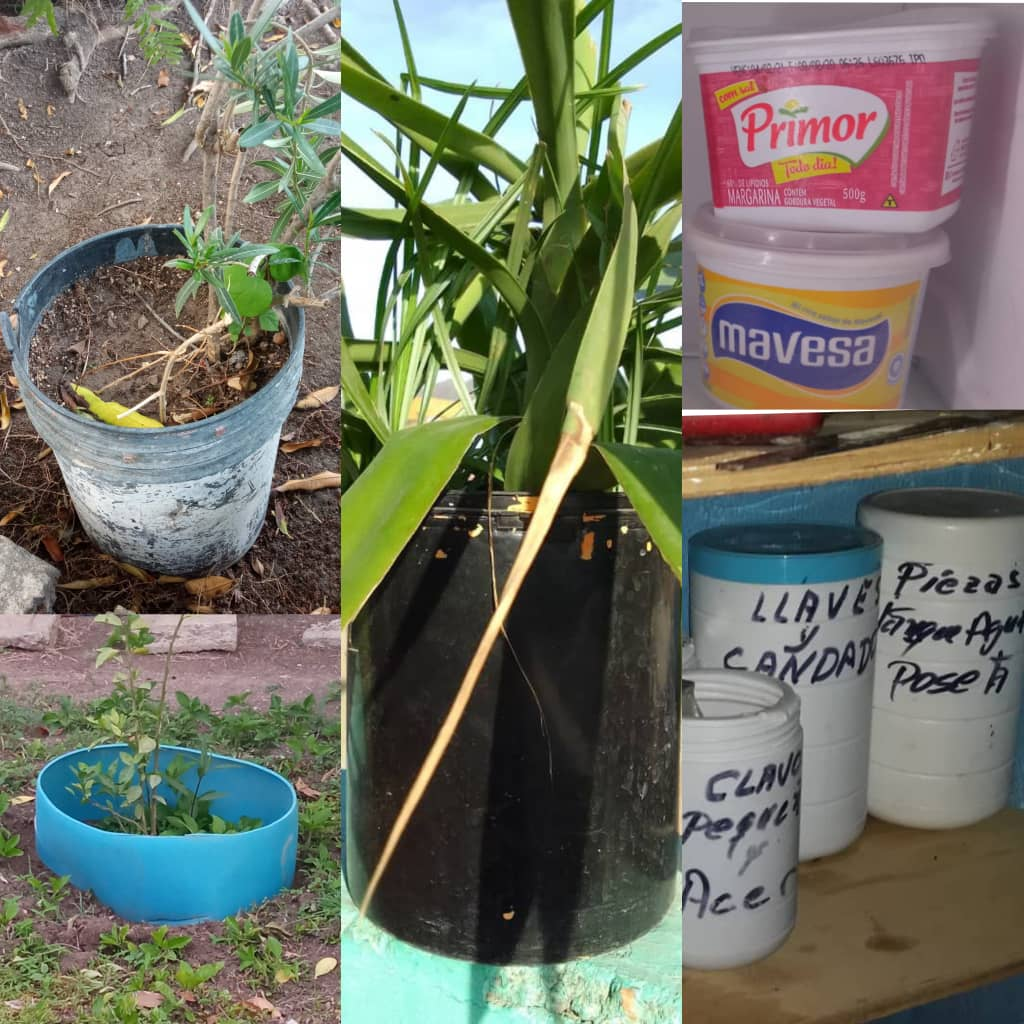
\includegraphics[width=15cm]{Media/Fotos/Foto 3 envases.jpeg}
    \label{fig:anexo7}
\end{figure}

\setlength{\parindent}{0ex}

Fuente: Elaboración propia

\newpage

\textbf{Anexo 8} \\
\textit{Reutilización de frascos para almacenar objetos}

\begin{figure}[!ht]
    \centering
    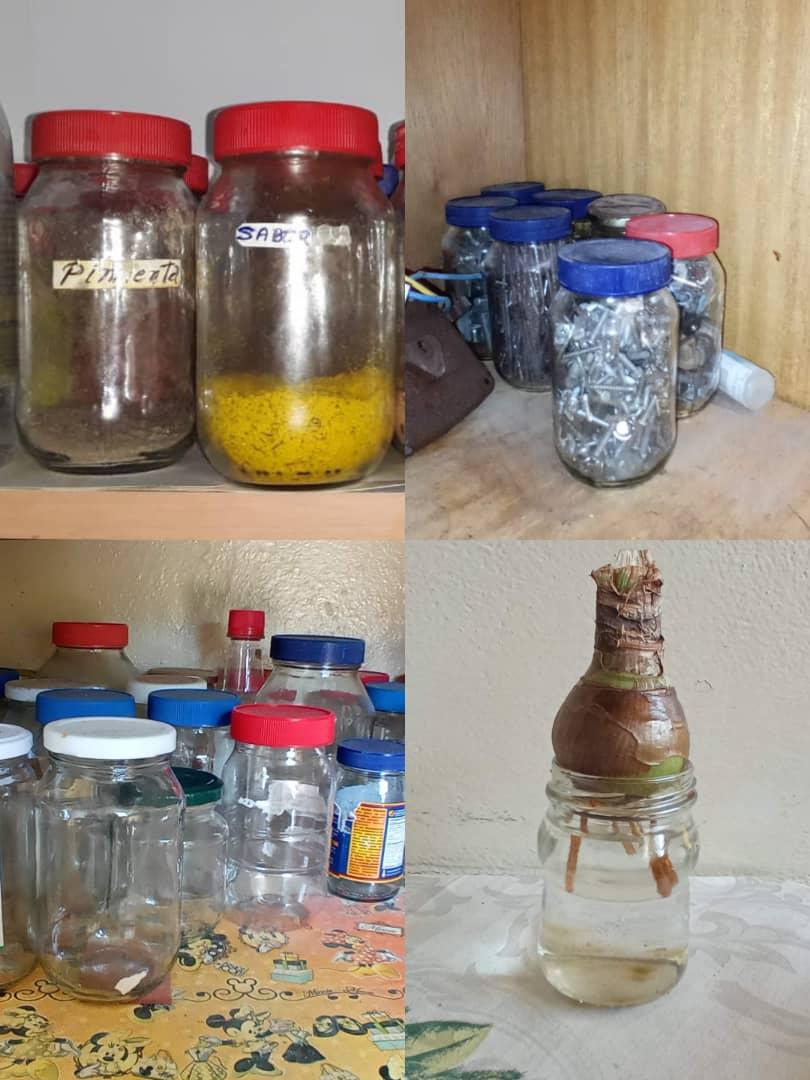
\includegraphics[width=15cm]{Media/Fotos/Foto 4 Frascos.jpeg}
    \label{fig:anexo9}
\end{figure}

\setlength{\parindent}{0ex}

Fuente: Elaboración propia

\newpage

\textbf{Anexo 9} \\
\textit{Elaboración de compost con desechos orgánicos}

\begin{figure}[!ht]
    \centering
    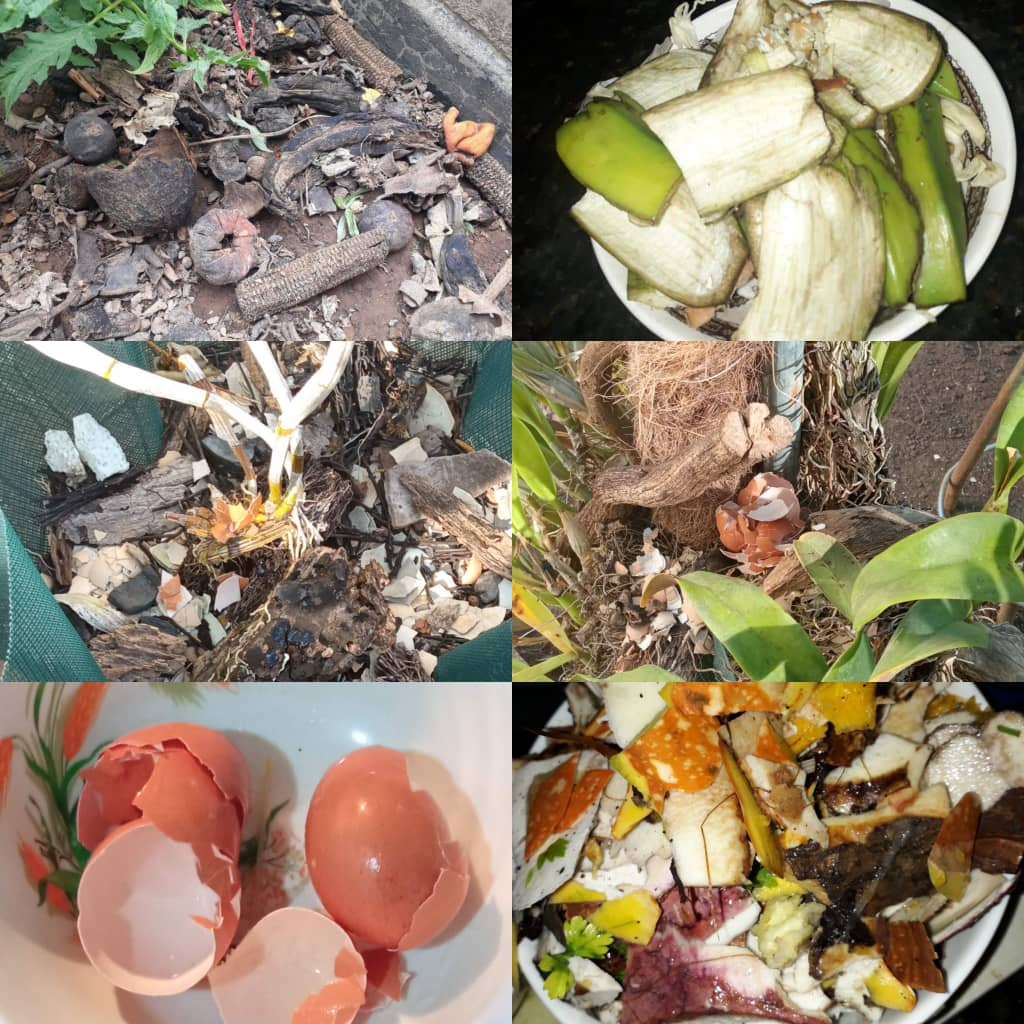
\includegraphics[width=15cm]{Media/Fotos/Foto 5 Compost.jpeg}
    \label{fig:anexo10}
\end{figure}

\setlength{\parindent}{0ex}

Fuente: Elaboración propia

\newpage

\textbf{Anexo 10} \\
\textit{Reutilización de hojas de papel}

\begin{figure}[!ht]
    \centering
    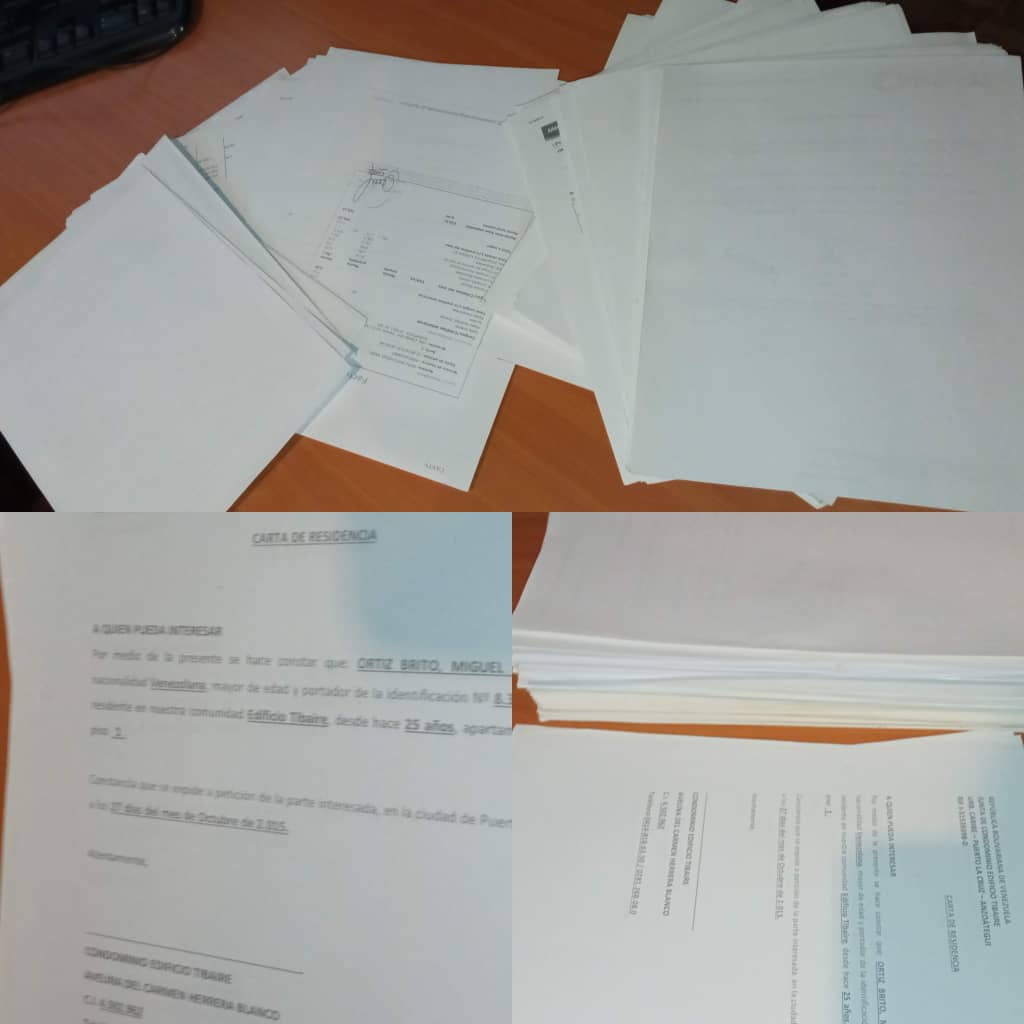
\includegraphics[width=15cm]{Media/Fotos/Foto 8 papel.jpeg}
    \label{fig:anexo11}
\end{figure}

\setlength{\parindent}{0ex}

Fuente: Elaboración propia

\newpage

\textbf{Anexo 11} \\
\textit{Clasificación casera de los desechos sólidos}

\begin{figure}[!ht]
    \centering
    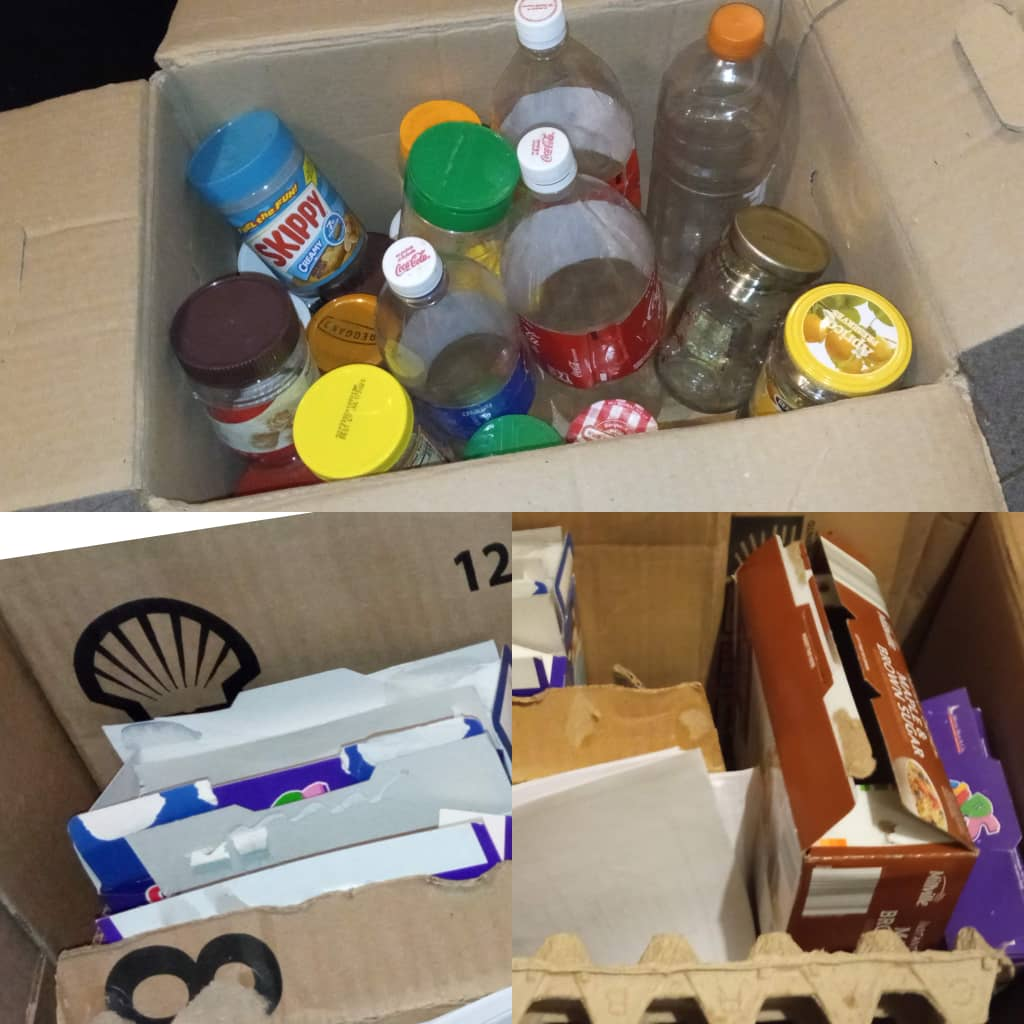
\includegraphics[width=15cm]{Media/Fotos/Foto final clasificacion.jpeg}
    \label{fig:anexo12}
\end{figure}

\setlength{\parindent}{0ex}

Fuente: Elaboración propia
